%!TEX root = slides.tex

\section{Bayesian Pharmacokinetic Modeling}

\subsection{Recommended References}
\begin{frame}{Bayesian Pharmacokinetic Modeling - Recommended References}
    \begin{vfilleditems}
        \item \textcite{Gabrielsson2006PKPDbook}:
        \begin{vfilleditems}
            \item Chapter 1: General Principles
            \item Chapter 2: Pharmacokinetic Concepts
        \end{vfilleditems}
        \item \textcite{Owen2014PKPDbook}:
        \begin{vfilleditems}
            \item Chapter 10: PK/PD Models
        \end{vfilleditems}
        \item \textcite{Bonate2011PKPDbook}:
        \begin{vfilleditems}
            \item Chapter 10: Bayesian Modeling regression
        \end{vfilleditems}
        \item \textcite{margossian2022torsten}
    \end{vfilleditems}
\end{frame}

\subsection{Pharmacokinetics}
\begin{frame}{Pharmacokinetics}
    \begin{defn}[Pharmacokinetics]
        \begin{quotation}
            Pharmacokinetics is the study of the time course of drug concentration in
            different body spaces such as plasma, blood, urine, cerebrospinal fluid, and
            tissues, and the relationship between concentration and the time course of
            drug action such as onset, intensity, and duration of action.
        \end{quotation}
        \vfill \vfill
        \textcite[13]{Gabrielsson2006PKPDbook}
    \end{defn}
\end{frame}

\begin{frame}{Pharmacokinetics}
    Pharmacokinetics is generally represented as \textbf{``PK'' compartments} in a model.
    \vfill
    They can be either:
    \begin{vfilleditems}
        \item \textbf{Pharmacokinetic} (PK) models with only PK compartments
        \item \textbf{Phamacokynetic-Pharmacodynamic}\footnote{more about these later on.} (PKPD) models with both PK compartments and PD compartments
    \end{vfilleditems}
\end{frame}

\subsection{Compartment Models}
\subsubsection{1-Compartment Model}
\begin{frame}{1-Compartment Model}
    $$
        \text{Central}^{\prime} = -\frac{CL}{V_C} \cdot \text{Central}
    $$
    where:
    \begin{vfilleditems}
        \item $CL$ is elimination clearance from the Central compartment
        \item $V_C$ is volume of the Central compartment
    \end{vfilleditems}
\end{frame}

\begin{frame}{1-compartment Model with First-Order Absorption}
    $$
        \begin{aligned}
            \text{Depot}^{\prime}   & =        -Ka \cdot \text{Depot}                                        \\
            \text{Central}^{\prime} & =  Ka \cdot \text{Depot}        & -\frac{CL}{V_C} \cdot \text{Central} \\
        \end{aligned}
    $$
    where:
    \begin{vfilleditems}
        \item $CL$ is elimination clearance from the Central compartment
        \item $V_C$ is volume of the Central compartment
        \item $Ka$ is absorption rate constant
    \end{vfilleditems}

\end{frame}

\subsubsection{2-Compartment Model}
\begin{frame}{2-Compartment Model}
    $$
        \begin{aligned}
            \text{Central}^{\prime}    & = -\frac{(CL + Q)}{V_C} & \cdot \text{Central} & + \frac{Q}{V_P} \cdot \text{Peripheral} \\
            \text{Peripheral}^{\prime} & =        \frac{Q}{V_C}  & \cdot \text{Central} & - \frac{Q}{V_P} \cdot \text{Peripheral}
        \end{aligned}
    $$
    where:
    \begin{vfilleditems}
        \item $CL$ is elimination clearance from the Central compartment
        \item $Q$ is the intercompartmental clearance
        \item $V_C$ is volume of the Central compartment
        \item $V_P$ is the volume of the Peripheral compartment
    \end{vfilleditems}
\end{frame}

\begin{frame}{2-Compartment Model with First-Order Absorption}
    $$
        \begin{aligned}
            \text{Depot}^{\prime}      & =        -Ka \cdot \text{Depot}                                                                                          \\
            \text{Central}^{\prime}    & =  Ka \cdot \text{Depot}        & -\frac{(CL + Q)}{V_C} & \cdot \text{Central} & + \frac{Q}{V_P} \cdot \text{Peripheral} \\
            \text{Peripheral}^{\prime} & =                               & \frac{Q}{V_C}         & \cdot \text{Central} & - \frac{Q}{V_P} \cdot \text{Peripheral}
        \end{aligned}
    $$
    where:
    \begin{vfilleditems}
        \item $CL$ is elimination clearance from the Central compartment
        \item $Q$ is the intercompartmental clearance
        \item $V_C$ is volume of the Central compartment
        \item $V_P$ is the volume of the Peripheral compartment
        \item $Ka$ is absorption rate constant
    \end{vfilleditems}
\end{frame}

\subsection{Bayesian PK Models}
\begin{frame}{How to make it Bayesian?}
    Just put \textbf{priors} in all parameters:
    $$
        \begin{aligned}
            CL  & \sim \text{LogNormal}(\log{\mu_{CL}}, \sigma_{CL})   \\
            Q   & \sim \text{LogNormal}(\log{\mu_{Q}}, \sigma_{Q})     \\
            V_C & \sim \text{LogNormal}(\log{\mu_{V_C}}, \sigma_{V_C}) \\
            V_P & \sim \text{LogNormal}(\log{\mu_{V_P}}, \sigma_{V_P}) \\
            Ka  & \sim \text{LogNormal}(\log{\mu_{Ka}}, \sigma_{Ka})
        \end{aligned}
    $$
\end{frame}

\subsection{Bayesian PK Models in Pumas}
\begin{frame}{Bayesian PK model in Pumas}
    \centering
    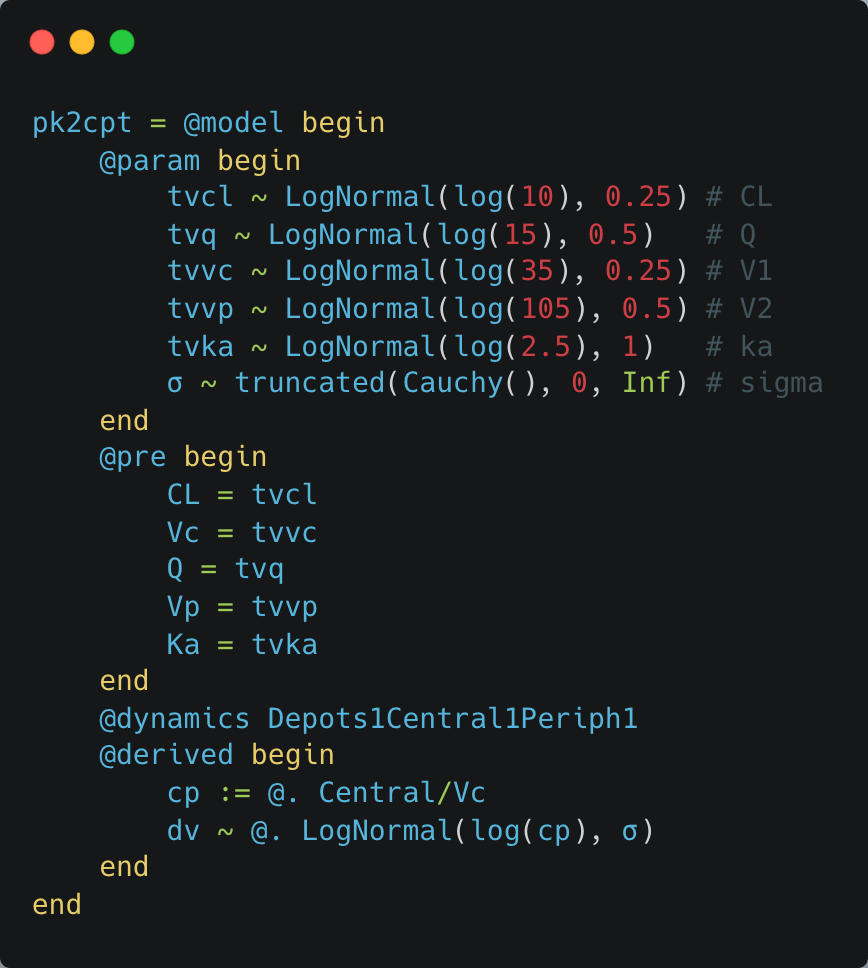
\includegraphics[width=0.4\columnwidth]{two_cmt_pk.png}
\end{frame}
